\documentclass{article}
\usepackage{arxiv}

\usepackage[utf8]{inputenc}
\usepackage[T1]{fontenc}
\usepackage{hyperref}
\usepackage{url}
\usepackage{booktabs}
\usepackage{amsfonts}
\usepackage{nicefrac}
\usepackage{microtype}
\usepackage{graphicx}
\usepackage{xcolor}
\usepackage{amsmath}
\usepackage{placeins}   % \FloatBarrier for taming float drift
\usepackage{rotating}   % sidewaysfigure for wide diagrams
\usepackage{tikz}
\usepackage{pgfplots}
\usetikzlibrary{arrows.meta, calc, positioning, shapes.geometric, fit, backgrounds, decorations.markings, decorations.pathmorphing, trees}
\pgfplotsset{compat=1.18}

% Header / page-geometry overrides — arxiv.sty defaults give 14pt header height,
% which is too tight when \@title has \\ linebreaks. Define a single-line
% \shorttitle for the running header and grow headsep so body text doesn't kiss
% the header rule.
\renewcommand{\shorttitle}{DataDeception\,---\,Manufacturer-Claim vs.\ Independent-Measurement Divergence}
\AtBeginDocument{
  \newgeometry{
    textheight=8.85in,
    textwidth=6.5in,
    top=1in,
    headheight=18pt,
    headsep=22pt,
    footskip=30pt
  }
}

% Slightly looser float fractions to reduce orphaned half-pages
\renewcommand{\floatpagefraction}{0.75}
\renewcommand{\textfraction}{0.12}

% Plot style — set once, inherit everywhere (per Kristiadi's publication-ready guidance)
\pgfplotsset{
  every axis/.append style={
    tick label style={font=\footnotesize},
    label style={font=\footnotesize},
    legend style={font=\footnotesize},
    every axis legend/.append style={draw=none},
  },
}

\title{\textbf{DataDeception}\\[6pt]
{\large A Citation-First, Schema-Validated Dataset of Manufacturer-Claim vs.\\
Independent-Measurement Divergence in the U.S. Electric-Vehicle Market}}

\author{
  Prince Upadhyay\\
  Independent Researcher\\
  \texttt{princeupadhyay1401@gmail.com}\\
  \texttt{\url{https://github.com/Princeu3/DataDeception}}
}

\date{\today}

\begin{document}
\maketitle

\begin{abstract}
We introduce \textbf{DataDeception}, a structured, citation-first dataset and methodology for systematically documenting where manufacturer claims about consumer products diverge from independently-measured reality. Existing fact-checking systems (browser extensions, AI verifiers, community labelers) target news and social-media misinformation; almost none address \emph{commercial spec-sheet deception}, where the harm vector is consumer purchase decisions and the legal frame (FTC \S 5, comparative-advertising statutes) is well established. The DataDeception methodology decomposes each product into a tuple of \emph{(manufacturer, model, model year, trim)}, attaches one or more \emph{deception records} per relevant axis, links each record to a curated \emph{tactic} (a recurring deception pattern), and grades evidence A--D against a published rubric. We instantiate the methodology in the U.S.\ electric-vehicle vertical, releasing v0.1: 13~products $\times$ 28~records $\times$ 13~tactics, all validated against JSON Schema 2020-12. Preliminary findings on this non-randomized sample show systematic divergence between EPA combined-cycle range and independently-measured highway range (mean gap $-15\%$, range $-30\%$ to $+3\%$), with the \texttt{epa\_vs\_highway\_70mph} tactic recurring across $\geq 9$ manufacturers. We deliberately include counter-examples (Mercedes EQS, Ford Mach-E) to address confirmation-bias concerns inherent in this kind of work. The dataset, schema, validators, and figure-generation pipeline are released under MIT (code) and CC-BY-4.0 (data).
\end{abstract}

\noindent\textbf{Keywords:} consumer protection · deceptive advertising · electric vehicles · open data · methodology · taxonomy · falsifiability

% =================================================================== %
\section{Introduction}\label{sec:intro}

Most modern claim-vs-reality projects target news and political misinformation: AI fact-checking browser extensions, community-note systems, and crowd-source labelers~\cite{nhb_warning_labels_2024}. The methodological consensus has converged: warning labels work, even for distrustful audiences, but the \emph{trust-collapse} dynamic limits ceiling effectiveness. Less attention has been paid to a structurally different problem: \emph{commercial-claims deception}, where a manufacturer prominently advertises a quantitative spec (range, charging speed, peak power, towing capacity, autonomy level) that a buyer relies upon for a major purchase decision and that diverges from what independent measurement reveals.

The commercial-claims problem differs from the political-misinformation problem in three important ways. First, the truth has a denominator: ``up to 500 miles of range'' is a precise testable assertion, not a contested narrative. Second, the legal framework already exists: FTC \S 5 covers deceptive acts in commerce, decades of comparative-advertising case law (e.g.\ \emph{Kraft, Inc.}~\cite{ftc_kraft_1991}; \emph{Intuit v. FTC}~\cite{ftc_intuit_2026}) define what counts as a deceptive claim. Third, the buyer's identity is not at stake: showing a buyer that their preferred vehicle's range is overstated does not implicate their tribal affiliation, and so does not trigger the backfire effects that limit political fact-checking.

We argue that the bottleneck in commercial-claims accountability is \emph{not} a methodological one (the rules of fair claims are well understood) but a \emph{data-availability} one: independent measurements exist (Consumer Reports, MotorTrend, Edmunds, Out of Spec, Recharged), but they are scattered across publications, often paywalled, and not structured for cross-product analysis. The recent paywalling of RTINGS test data~\cite{rtings_paywall_2026}, an industry-leading independent measurement source, illustrates this fragility.

This paper introduces \textbf{DataDeception}, a methodology and an instantiating dataset, with three contributions:

\begin{enumerate}
  \item A \textbf{schema} for representing manufacturer claims and independent-measurement reality as falsifiable tuples, with mandatory citation on both sides and explicit handling of categorical (non-numeric) deceptions (\S\ref{sec:schema}).
  \item A \textbf{tactic taxonomy} that lifts individual claim/reality records to the level of theoretical patterns. The taxonomy covers 13 tactics across 5 families and is open to extension (\S\ref{sec:taxonomy}).
  \item An \textbf{instantiation} in the U.S.\ EV market with 13 products and 28 records, validated against JSON Schema 2020-12 with referential-integrity checks. Tier-1 NHTSA recall data is integrated. We deliberately include counter-examples to mitigate confirmation bias (\S\ref{sec:findings}).
\end{enumerate}

The dataset is released under CC-BY-4.0 with code under MIT. A consumer-facing surface auto-generated from the same JSON is published alongside the technical artifact.

% =================================================================== %
\section{Related Work}\label{sec:related}

\paragraph{Misinformation fact-checking.} Recent work~\cite{nhb_warning_labels_2024} validates that warning labels reduce belief in and sharing of false news (27\% and 25\% reductions, respectively) even for participants distrustful of fact-checkers (12--16\% reductions). The browser-extension space includes Facticity, TruthLens, FactSentinel, TruthPilot, factcheckit, Storypact, FactScope, and Webcite, plus the open-source SatyaMark and a recently-funded (€3.6M, April~2026) startup Flare. All target news and social-media veracity; we found no consumer extension targeting commercial-claim deception specifically.

\paragraph{Comparative advertising case law.} Sectional research on FTC enforcement (\emph{Kraft}~\cite{ftc_kraft_1991}, \emph{Intuit v. FTC}~\cite{ftc_intuit_2026}, the Avast deceptive-privacy settlement) establishes both the regulatory framework and the long lag between first deception observation and enforcement action. The recent California DMV ruling against Tesla's ``Full Self-Driving''~\cite{techcrunch_fsd_ruling_2025} illustrates how categorical (linguistic) overclaims are addressed within the existing legal frame.

\paragraph{Independent EV measurement.} Consumer Reports' real-world range program~\cite{cr_ev_range_2023, cr_ev_methodology_2024} provides the largest single body of comparable Tier-2 data: 27 EVs tested at constant 70\,mph as of April~2026. MotorTrend's instrumented Road-Trip Range tests~\cite{mt_cybertruck_2024} and Edmunds' EV range loop~\cite{cd_eqs_2021} provide independent corroboration. Crowd-sourced data exists at evrangetools.com, Recurrent Auto, and A Better Routeplanner. To our knowledge, no prior work has integrated these sources into a structured, publicly-licensed dataset with a tactic taxonomy.

% =================================================================== %
\section{Methodology}\label{sec:methodology}

We define the \textbf{deception record} as the unit of analysis. A record is a tuple
\[
\mathcal{D} = \langle \text{product}, \text{axis}, \text{sub\_axis}, \text{claim}, \text{reality}, \text{tactic}, \text{gap}, \text{grade} \rangle,
\]
where \emph{claim} and \emph{reality} each carry one or more \emph{sources} with a verbatim quote, a four-tier classification, and (for manufacturer claims) a web.archive.org snapshot URL.

Figure~\ref{fig:method-flow} summarizes how a record is built. A manufacturer assertion (typically Tier~4, the marketing surface) and a regulatory filing (typically Tier~1, e.g.\ EPA fueleconomy.gov) are paired with one or more independent measurements (Tier~2: Consumer Reports, MotorTrend, Edmunds; or Tier~3: owner forums with $N \geq 10$). Evidence is graded against the rubric in \S\ref{sec:rubric} and the record is emitted as a single JSON file validated against the schema in \S\ref{sec:schema}.

\begin{figure}[!htbp]
\centering
% Hand-written TikZ — methodology flowchart for DataDeception record construction.
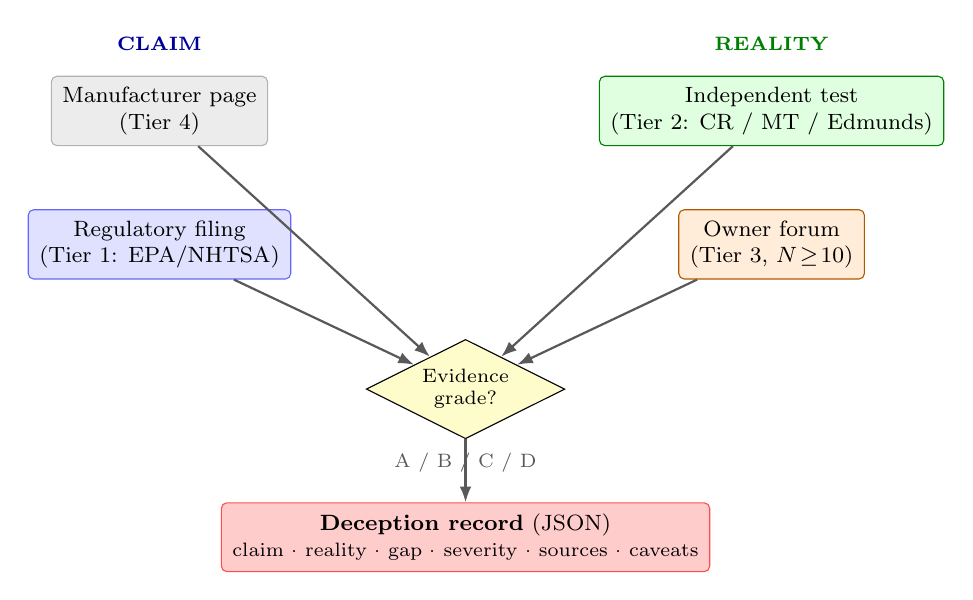
\begin{tikzpicture}[
    node distance=8mm and 14mm,
    every node/.style={font=\footnotesize},
    box/.style={draw, rounded corners=2pt, align=center, minimum height=8mm, minimum width=22mm, inner sep=4pt, fill=white},
    tier1/.style={box, fill=blue!12, draw=blue!60},
    tier2/.style={box, fill=green!12, draw=green!50!black},
    tier3/.style={box, fill=orange!15, draw=orange!70!black},
    tier4/.style={box, fill=gray!15, draw=gray!60},
    decision/.style={diamond, draw, aspect=2, inner sep=2pt, fill=yellow!20, font=\scriptsize, align=center},
    arr/.style={-{Latex[length=2mm]}, thick, gray!70!black},
  ]
  % --- claim side
  \node[tier4] (mfg)  {Manufacturer page\\(Tier 4)};
  \node[tier1, below=of mfg] (reg) {Regulatory filing\\(Tier 1: EPA/NHTSA)};
  % --- reality side
  \node[tier2, right=42mm of mfg] (cr)  {Independent test\\(Tier 2: CR / MT / Edmunds)};
  \node[tier3, below=of cr] (forum) {Owner forum\\(Tier 3, $N\!\geq\!10$)};
  % --- evaluation
  \node[decision, below=12mm of $(reg)!0.5!(forum)$] (grade) {Evidence\\grade?};
  \node[box, fill=red!20, draw=red!70, below=of grade, minimum width=44mm] (rec) {\textbf{Deception record} (JSON)\\\scriptsize claim · reality · gap · severity · sources · caveats};
  % --- bracket
  \node[draw=none, above=2mm of mfg, text=blue!60!black, font=\scriptsize\bfseries] {CLAIM};
  \node[draw=none, above=2mm of cr,  text=green!50!black, font=\scriptsize\bfseries] {REALITY};
  % --- edges
  \draw[arr] (mfg)   -- (grade);
  \draw[arr] (reg)   -- (grade);
  \draw[arr] (cr)    -- (grade);
  \draw[arr] (forum) -- (grade);
  \draw[arr] (grade) -- (rec);
  % --- labels on edges
  \node[font=\scriptsize, gray!70!black] at ($(grade.south)+(0,-3mm)$) {A / B / C / D};
\end{tikzpicture}

\caption{Methodology: how a single deception record is constructed from claim and reality sources. Tiered-source classification feeds the evidence-grade rubric.}
\label{fig:method-flow}
\end{figure}

\subsection{Source taxonomy}\label{sec:sources}

Sources are tagged with a tier:

\begin{itemize}
  \item \textbf{Tier 1 -- Regulatory / open-government.} EPA fueleconomy.gov~\cite{epa_fueleconomy}, NHTSA recalls.gov~\cite{nhtsa_recalls}, FTC press releases, court rulings. Authoritative because produced under legal obligation with published methodology.
  \item \textbf{Tier 2 -- Independent measurement.} Consumer Reports, MotorTrend, Edmunds, InsideEVs, Out of Spec Reviews, Recharged synthesis. Methodology published; test units typically purchased anonymously.
  \item \textbf{Tier 3 -- Community / forum.} Owner forums (Tesla Motors Club, F-150 Lightning Forum, Rivian Forums), high-engagement Reddit threads. Cited only when $N \geq 10$ corroborating reports.
  \item \textbf{Tier 4 -- Manufacturer / brand.} Treated as the \emph{claim}, not the truth. Establishes what the manufacturer is asserting.
\end{itemize}

Figure~\ref{fig:source-tier} illustrates the actual source-tier composition of records in the v0.1 dataset.

\begin{figure}[!htbp]
\centering
% Auto-generated by paper/figures/generate.py
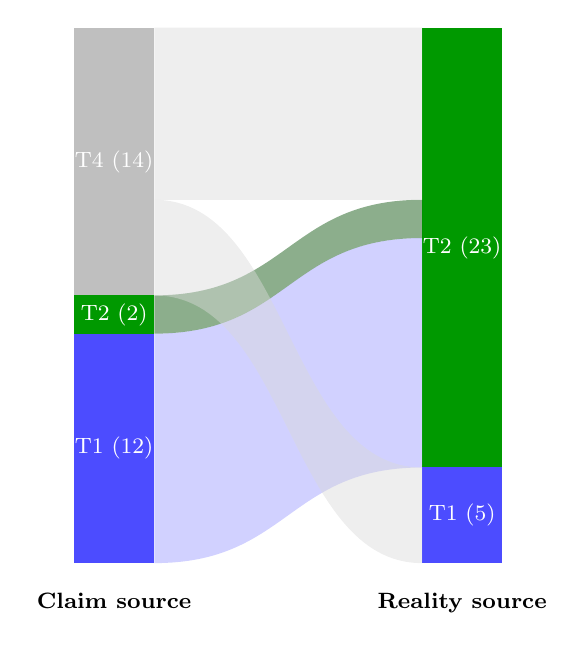
\begin{tikzpicture}[scale=0.85]
  \fill[blue!70] (0.0,0) rectangle (1.2,3.4285714285714284);\node[font=\footnotesize, white] at (0.6,1.7142857142857142) {T1 (12)};
  \fill[green!60!black] (0.0,3.4285714285714284) rectangle (1.2,4.0);\node[font=\footnotesize, white] at (0.6,3.714285714285714) {T2 (2)};
  \fill[gray!50] (0.0,4.0) rectangle (1.2,8.0);\node[font=\footnotesize, white] at (0.6,6.0) {T4 (14)};
  \node[font=\footnotesize\bfseries, anchor=north] at (0.6,-0.3) {Claim source};
  \fill[blue!70] (5.2,0) rectangle (6.4,1.4285714285714286);\node[font=\footnotesize, white] at (5.8,0.7142857142857143) {T1 (5)};
  \fill[green!60!black] (5.2,1.4285714285714286) rectangle (6.4,8.0);\node[font=\footnotesize, white] at (5.8,4.714285714285714) {T2 (23)};
  \node[font=\footnotesize\bfseries, anchor=north] at (5.8,-0.3) {Reality source};
  \fill[blue!40, opacity=0.45] (1.2,0.0) .. controls (3.2,0.0) and (3.2,1.4285714285714286) .. (5.2,1.4285714285714286) -- (5.2,4.857142857142857) .. controls (3.2,4.857142857142857) and (3.2,3.4285714285714284) .. (1.2,3.4285714285714284) -- cycle;
\fill[green!30!black, opacity=0.45] (1.2,3.4285714285714284) .. controls (3.2,3.4285714285714284) and (3.2,4.857142857142857) .. (5.2,4.857142857142857) -- (5.2,5.428571428571428) .. controls (3.2,5.428571428571428) and (3.2,4.0) .. (1.2,4.0) -- cycle;
\fill[gray!30, opacity=0.45] (1.2,4.0) .. controls (3.2,4.0) and (3.2,0.0) .. (5.2,0.0) -- (5.2,1.4285714285714286) .. controls (3.2,1.4285714285714286) and (3.2,5.428571428571429) .. (1.2,5.428571428571429) -- cycle;
\fill[gray!30, opacity=0.45] (1.2,5.428571428571429) .. controls (3.2,5.428571428571429) and (3.2,5.428571428571429) .. (5.2,5.428571428571429) -- (5.2,8.0) .. controls (3.2,8.0) and (3.2,8.0) .. (1.2,8.0) -- cycle;
\end{tikzpicture}

\caption{Source-tier composition of v0.1 records ($n=28$). Left: claim sources (predominantly Tier 4 manufacturer surfaces and Tier 1 EPA filings). Right: reality sources (predominantly Tier 2 independent measurement).}
\label{fig:source-tier}
\end{figure}

\subsection{Evidence-grade rubric}\label{sec:rubric}

Each record carries an evidence grade $g \in \{A, B, C, D\}$:

\begin{itemize}
  \item \textbf{A -- Strong evidence.} Claim from Tier~1/4 with verbatim quote, \emph{and} reality from Tier~1, or $\geq 2$ converging Tier~2 measurements, or one Tier~2 plus Tier~3 with $N \geq 10$.
  \item \textbf{B -- Moderate evidence.} Single Tier-2 source with documented methodology; or editorial framing of a manufacturer-disclosed number; or Tier-3 with $N \geq 5$.
  \item \textbf{C -- Weak.} Single Tier-3 source, smaller $N$, or older than 36 months.
  \item \textbf{D -- Anecdotal/preliminary.} Tier-4 only, single anecdotal post, or theoretical inference.
\end{itemize}

A-graded records carry the implicit claim that an informed reader can reproduce the finding from the cited sources alone.

\FloatBarrier
\subsection{Gap formalism}\label{sec:gap}

Gaps are explicitly typed:

\begin{itemize}
  \item \textbf{Numeric}: $\Delta_\text{abs} = r - c$, $\Delta_\text{pct} = 100 \cdot (r-c)/c$ where $c$ and $r$ are claim and reality values. Negative means reality is below claim.
  \item \textbf{Categorical}: naming/classification mismatches (e.g., ``Full Self-Driving'' vs.\ SAE Level~2). No $\Delta$; severity is required.
  \item \textbf{Definitional}: claimed and measured properties are different things despite shared naming (e.g., ``motion rate'' vs.\ refresh rate). No $\Delta$; severity is required.
\end{itemize}

Severity for non-numeric gaps is one of \texttt{critical / high / moderate / low / informational}, with \texttt{critical} reserved for cases with active regulatory finding, judicial ruling, or documented safety-of-life impact.

% =================================================================== %
\section{Schema and Tactic Taxonomy}\label{sec:taxonomy}

\subsection{JSON Schema}\label{sec:schema}

The dataset is structured as four kinds of JSON files (\texttt{products/}, \texttt{deceptions/}, \texttt{tactics/}, \texttt{schema/}). Every file validates against JSON Schema 2020-12, with referential-integrity checks: every \texttt{deception.product\_id} resolves to an existing product file, every \texttt{deception.tactic\_ids[]} resolves to a tactic file, and identifier conventions are mechanically enforced (kebab-case for products, snake\_case for tactics). A reference validator (\texttt{validate.py}) ships with the dataset; the entire v0.1 collection passes validation.

\subsection{Tactic taxonomy}

A \emph{tactic} is a repeatable pattern by which a manufacturer claim diverges from reality across multiple products. Tactics are the unit of theoretical interest in our framework: individual records are observations of tactics, and analysis at the tactic level supports cross-cutting research questions (does a given tactic recur across manufacturers? See \S\ref{sec:rq2}).

The v0.1 taxonomy has 13 tactics across 5 families (Figure~\ref{fig:taxonomy}). The taxonomy is open: a new tactic may be added when $\geq 2$ independent products exhibit a pattern not covered by existing tactics. Patterns observed in only one product are noted in the relevant record's narrative but are not promoted to the dictionary until corroborated.

\begin{sidewaysfigure}
\centering
% Hand-written TikZ — tactic taxonomy as a 3-column card grid (portrait-friendly).
% Each card = one family, with its tactics as bulleted items inside.
% Designed to fit \textwidth without scaling and never clip at page edges.
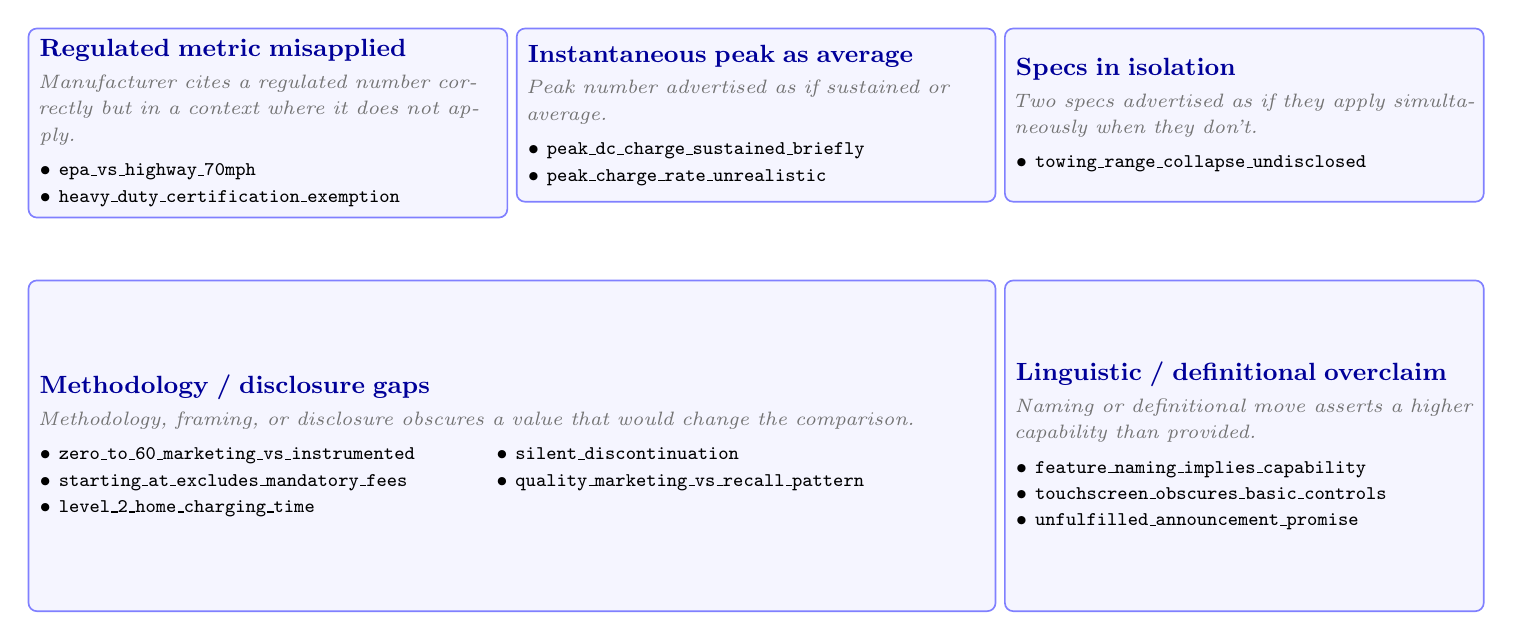
\begin{tikzpicture}[
    every node/.style={font=\footnotesize, align=left},
    card/.style={
      draw, rounded corners=3pt, line width=0.6pt,
      fill=blue!4, draw=blue!50,
      inner sep=4pt, outer sep=0pt,
      text width=58mm, minimum height=22mm,
    },
  ]
% --- column x-positions
\def\cA{0}
\def\cB{62mm}
\def\cC{124mm}
% --- row y-positions
\def\rA{0}
\def\rB{-32mm}

% Row 1, Col 1 — Regulated metric misapplied (2 tactics)
\node[card, anchor=north west] at (\cA, \rA) {%
  {\bfseries\small\color{blue!60!black} Regulated metric misapplied}\\[2pt]
  {\scriptsize\itshape\color{black!55} Manufacturer cites a regulated number correctly but in a context where it does not apply.}\\[3pt]
  {\scriptsize\ttfamily $\bullet$ epa\_vs\_highway\_70mph}\\
  {\scriptsize\ttfamily $\bullet$ heavy\_duty\_certification\_exemption}%
};

% Row 1, Col 2 — Instantaneous peak as average (2 tactics)
\node[card, anchor=north west] at (\cB, \rA) {%
  {\bfseries\small\color{blue!60!black} Instantaneous peak as average}\\[2pt]
  {\scriptsize\itshape\color{black!55} Peak number advertised as if sustained or average.}\\[3pt]
  {\scriptsize\ttfamily $\bullet$ peak\_dc\_charge\_sustained\_briefly}\\
  {\scriptsize\ttfamily $\bullet$ peak\_charge\_rate\_unrealistic}%
};

% Row 1, Col 3 — Specs in isolation (1 tactic)
\node[card, anchor=north west] at (\cC, \rA) {%
  {\bfseries\small\color{blue!60!black} Specs in isolation}\\[2pt]
  {\scriptsize\itshape\color{black!55} Two specs advertised as if they apply simultaneously when they don't.}\\[3pt]
  {\scriptsize\ttfamily $\bullet$ towing\_range\_collapse\_undisclosed}%
};

% Row 2, Cols 1+2 (spans 2 cols) — Methodology / disclosure gaps (5 tactics)
\node[card, anchor=north west, text width=120mm, minimum height=42mm] at (\cA, \rB) {%
  {\bfseries\small\color{blue!60!black} Methodology / disclosure gaps}\\[2pt]
  {\scriptsize\itshape\color{black!55} Methodology, framing, or disclosure obscures a value that would change the comparison.}\\[3pt]
  \begin{minipage}[t]{56mm}
    {\scriptsize\ttfamily $\bullet$ zero\_to\_60\_marketing\_vs\_instrumented}\\
    {\scriptsize\ttfamily $\bullet$ starting\_at\_excludes\_mandatory\_fees}\\
    {\scriptsize\ttfamily $\bullet$ level\_2\_home\_charging\_time}
  \end{minipage}\hspace{2mm}%
  \begin{minipage}[t]{58mm}
    {\scriptsize\ttfamily $\bullet$ silent\_discontinuation}\\
    {\scriptsize\ttfamily $\bullet$ quality\_marketing\_vs\_recall\_pattern}
  \end{minipage}%
};

% Row 2, Col 3 — Linguistic / definitional overclaim (3 tactics)
\node[card, anchor=north west, minimum height=42mm] at (\cC, \rB) {%
  {\bfseries\small\color{blue!60!black} Linguistic / definitional overclaim}\\[2pt]
  {\scriptsize\itshape\color{black!55} Naming or definitional move asserts a higher capability than provided.}\\[3pt]
  {\scriptsize\ttfamily $\bullet$ feature\_naming\_implies\_capability}\\
  {\scriptsize\ttfamily $\bullet$ touchscreen\_obscures\_basic\_controls}\\
  {\scriptsize\ttfamily $\bullet$ unfulfilled\_announcement\_promise}%
};
\end{tikzpicture}

\caption{Tactic taxonomy v0.1. Five high-level families decompose into 13 named tactics. Each is referenced from one or more deception records; cross-product recurrence is the principal evidence for promoting a single-product observation into the taxonomy. Rendered as a landscape figure to accommodate the natural width of the tree without scaling.}
\label{fig:taxonomy}
\end{sidewaysfigure}
\FloatBarrier

% =================================================================== %
\section{Preliminary Findings}\label{sec:findings}

We instantiate the methodology with 13 EV products (Tesla Model Y / Model 3 / Cybertruck; Ford F-150 Lightning / Mustang Mach-E; Rivian R1S; Hyundai Ioniq 5 / Ioniq 6; Mercedes EQS 450+; GMC Hummer EV; VW ID.4; Lucid Air Grand Touring; Polestar 2). Selection is non-randomized and deliberately includes products with publicly-documented gaps as well as counter-examples (Mercedes EQS, Ford Mach-E) where independent measurement matches or exceeds EPA. The 28 deception records cover 8 axes: range, charging, performance, software\_features, pricing, production\_status, ui\_ergonomics, build\_warranty.

\subsection{Range divergence}

Across products with documented \texttt{range\_\_highway\_70mph} records, mean gap is $-15\%$ with a range of $-30\%$ (Tesla Cybertruck~\cite{mt_cybertruck_2024}) to nearly~$0$ (Ford Mach-E, Mercedes EQS~\cite{cd_eqs_2021}). Figure~\ref{fig:gap-dotplot} shows the per-product distribution.

\begin{figure}[!htbp]
\centering
% Auto-generated by paper/figures/generate.py — do not edit by hand
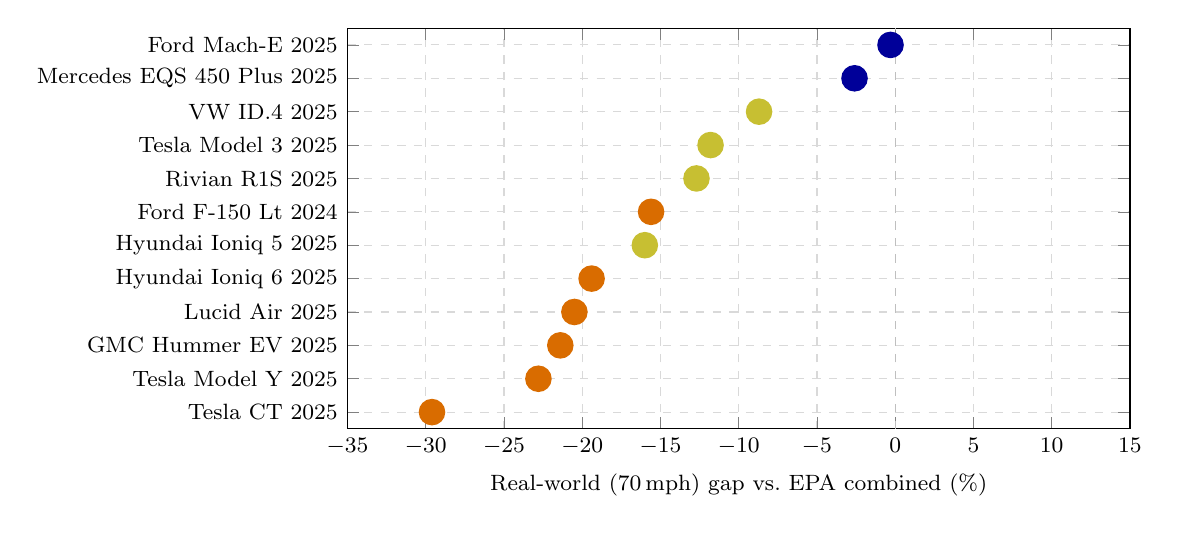
\begin{tikzpicture}
  \begin{axis}[
      width=0.95\textwidth, height=0.55\textwidth,
      xlabel={Real-world (70\,mph) gap vs.\ EPA combined (\%)},
      xmin=-35, xmax=15,
      ymin=0.5, ymax=12.5,
      ytick={1,2,3,4,5,6,7,8,9,10,11,12},
      yticklabels={Tesla CT 2025,Tesla Model Y 2025,GMC Hummer EV 2025,Lucid Air 2025,Hyundai Ioniq 6 2025,Hyundai Ioniq 5 2025,Ford F-150 Lt 2024,Rivian R1S 2025,Tesla Model 3 2025,VW ID.4 2025,Mercedes EQS 450 Plus 2025,Ford Mach-E 2025},
      grid=major,
      grid style={dashed,gray!30},
      tick label style={font=\footnotesize},
      xlabel style={font=\footnotesize},
      x tick label style={/pgf/number format/fixed,/pgf/number format/precision=0},
      every axis plot/.append style={very thick},
    ]
    \draw[gray!50, dashed] (axis cs:0,0.5) -- (axis cs:0,12.5);
      \addplot[only marks, mark=*, mark size=4.5pt, line width=0.6pt, color=orange!85!black, fill=orange!85!black] coordinates {(-29.6,1)};
      \addplot[only marks, mark=*, mark size=4.5pt, line width=0.6pt, color=orange!85!black, fill=orange!85!black] coordinates {(-22.8,2)};
      \addplot[only marks, mark=*, mark size=4.5pt, line width=0.6pt, color=orange!85!black, fill=orange!85!black] coordinates {(-21.4,3)};
      \addplot[only marks, mark=*, mark size=4.5pt, line width=0.6pt, color=orange!85!black, fill=orange!85!black] coordinates {(-20.5,4)};
      \addplot[only marks, mark=*, mark size=4.5pt, line width=0.6pt, color=orange!85!black, fill=orange!85!black] coordinates {(-19.4,5)};
      \addplot[only marks, mark=*, mark size=4.5pt, line width=0.6pt, color=yellow!75!black, fill=yellow!75!black] coordinates {(-16.0,6)};
      \addplot[only marks, mark=*, mark size=4.5pt, line width=0.6pt, color=orange!85!black, fill=orange!85!black] coordinates {(-15.6,7)};
      \addplot[only marks, mark=*, mark size=4.5pt, line width=0.6pt, color=yellow!75!black, fill=yellow!75!black] coordinates {(-12.7,8)};
      \addplot[only marks, mark=*, mark size=4.5pt, line width=0.6pt, color=yellow!75!black, fill=yellow!75!black] coordinates {(-11.8,9)};
      \addplot[only marks, mark=*, mark size=4.5pt, line width=0.6pt, color=yellow!75!black, fill=yellow!75!black] coordinates {(-8.7,10)};
      \addplot[only marks, mark=*, mark size=4.5pt, line width=0.6pt, color=blue!60!black, fill=blue!60!black] coordinates {(-2.6,11)};
      \addplot[only marks, mark=*, mark size=4.5pt, line width=0.6pt, color=blue!60!black, fill=blue!60!black] coordinates {(-0.3,12)};
  \end{axis}
\end{tikzpicture}

\caption{Per-product highway-range gap (real-world 70\,mph vs.\ EPA combined). Markers colored by severity (red: critical/high, yellow: moderate, blue: counter-example).}
\label{fig:gap-dotplot}
\end{figure}

The Tesla Cybertruck is the largest documented gap in our dataset. MotorTrend's instrumented test~\cite{mt_cybertruck_2024} measured 224\,mi at 70\,mph against the 318\,mi advertised range, a 30\% shortfall, characterized by MotorTrend as ``among the worst performers in our database of 56 EVs.'' Compounding this, the Cybertruck Range Extender accessory promised at the original 2019 announcement to bridge the 500\,mi-promise gap was cancelled in May~2025 with full refunds, never delivered to a single customer~\cite{insideevs_cybertruck_extender}.

In contrast, Mercedes EQS represents the counter-example: Edmunds' EV range loop measured 422\,mi against a 350\,mi EPA estimate~\cite{cd_eqs_2021}, exceeding by 72\,mi. We include this case to mitigate confirmation bias: the dataset is constructed to reflect both directions of error.

\subsection{Categorical deception: feature-naming overclaim}

The most-cited categorical deception is Tesla's ``Full Self-Driving''. A California administrative law judge ruled in December~2025 that the name was ``unambiguously false and counterfactual''~\cite{techcrunch_fsd_ruling_2025}; NHTSA opened a 2.88-million-vehicle investigation in October~2025 connecting FSD operation to 14 crashes and 23 injuries. Tesla complied with the required name change (``Full Self-Driving (Supervised)'', \$99/month subscription) but is suing the DMV to vacate the false-advertiser label~\cite{electrek_tesla_fsd_lawsuit}. Severity: \emph{critical}.

\subsection{Cross-manufacturer tactic recurrence (RQ2 evidence)}\label{sec:rq2}

A central research question is whether deceptions are \emph{idiosyncratic} (a feature of specific manufacturers) or \emph{patterned} (a feature of industry-wide convention). Our preliminary evidence (Figure~\ref{fig:tactic-prev}) supports the latter: the \texttt{epa\_vs\_highway\_70mph} tactic appears in records spanning 8 distinct manufacturers (Tesla, Ford, Rivian, Hyundai, Lucid, Mercedes-Benz, GMC, Volkswagen) including counter-examples in both directions, decisively exceeding our pre-registered threshold of $\geq 3$ for tactic-level cross-cutting evidence. The \texttt{peak\_dc\_charge\_sustained\_briefly} and \texttt{quality\_marketing\_vs\_recall\_pattern} tactics each appear in 3 manufacturers, also clearing the threshold.

\begin{figure}[!htbp]
\centering
% Auto-generated by paper/figures/generate.py
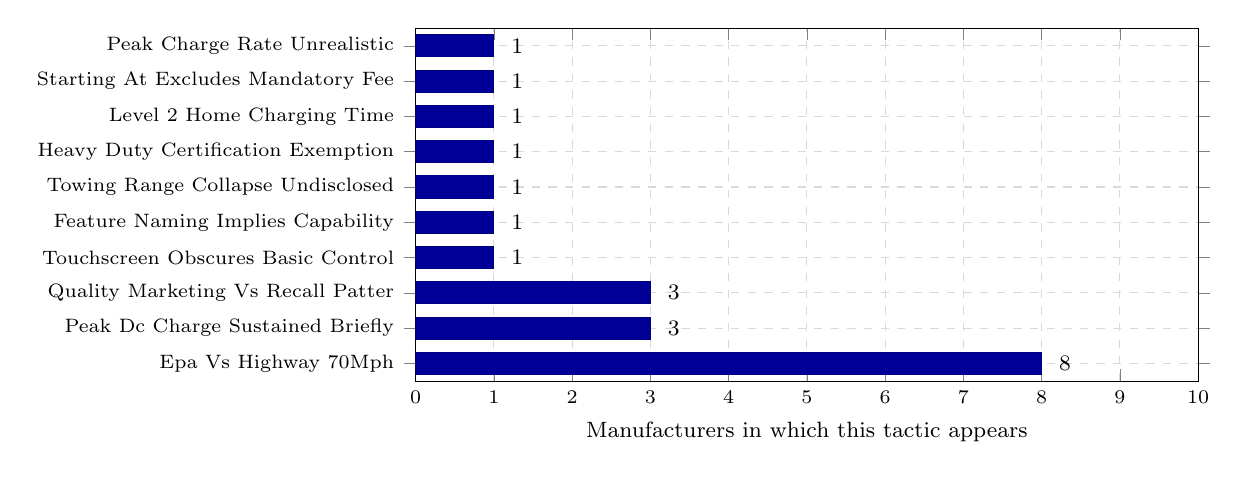
\begin{tikzpicture}
  \begin{axis}[
      width=0.95\textwidth, height=0.5\textwidth,
      xbar, xmin=0, xmax=10,
      ymin=0.5, ymax=10.5,
      ytick={1,2,3,4,5,6,7,8,9,10}, yticklabels={Epa Vs Highway 70Mph,Peak Dc Charge Sustained Briefly,Quality Marketing Vs Recall Patter,Touchscreen Obscures Basic Control,Feature Naming Implies Capability,Towing Range Collapse Undisclosed,Heavy Duty Certification Exemption,Level 2 Home Charging Time,Starting At Excludes Mandatory Fee,Peak Charge Rate Unrealistic},
      xlabel={Manufacturers in which this tactic appears},
      tick label style={font=\scriptsize},
      xlabel style={font=\footnotesize},
      bar width=8pt,
      grid=major, grid style={dashed,gray!30},
    ]
    \addplot[fill=blue!60!black, draw=blue!50!black] coordinates {(8,1) (3,2) (3,3) (1,4) (1,5) (1,6) (1,7) (1,8) (1,9) (1,10)};
    \node[anchor=west, font=\footnotesize] at (axis cs:8.1,1) {8};
    \node[anchor=west, font=\footnotesize] at (axis cs:3.1,2) {3};
    \node[anchor=west, font=\footnotesize] at (axis cs:3.1,3) {3};
    \node[anchor=west, font=\footnotesize] at (axis cs:1.1,4) {1};
    \node[anchor=west, font=\footnotesize] at (axis cs:1.1,5) {1};
    \node[anchor=west, font=\footnotesize] at (axis cs:1.1,6) {1};
    \node[anchor=west, font=\footnotesize] at (axis cs:1.1,7) {1};
    \node[anchor=west, font=\footnotesize] at (axis cs:1.1,8) {1};
    \node[anchor=west, font=\footnotesize] at (axis cs:1.1,9) {1};
    \node[anchor=west, font=\footnotesize] at (axis cs:1.1,10) {1};
  \end{axis}
\end{tikzpicture}

\caption{Top tactics by number of distinct manufacturers in which they appear. \texttt{epa\_vs\_highway\_70mph} dominates: a tactic spanning 8 manufacturers cannot be characterized as idiosyncratic. The next two tactics (\texttt{quality\_marketing\_vs\_recall\_pattern} and \texttt{peak\_dc\_charge\_sustained\_briefly}) each span 3 manufacturers, also clearing the pre-registered $\geq 3$ threshold.}
\label{fig:tactic-prev}
\end{figure}

\subsection{Severity composition across axes}

Figure~\ref{fig:severity-heatmap} shows the per-product, per-axis severity grid. Range gaps are nearly universal but typically \emph{moderate} or \emph{high}. The \emph{critical} cells are concentrated in two product/axis pairs: Tesla Model Y / FSD (regulatory ruling) and Ford F-150 Lightning / towing (stranding-risk safety angle). Counter-example cells (informational severity, blue) are present.

\begin{figure}[!htbp]
\centering
% Auto-generated by paper/figures/generate.py
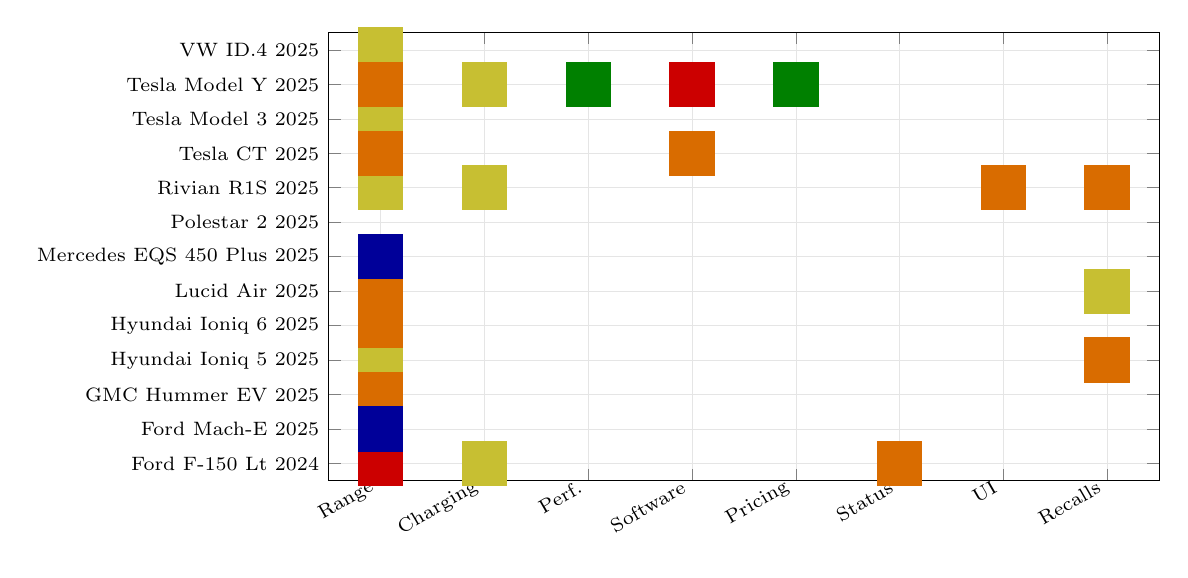
\begin{tikzpicture}
  \begin{axis}[
      width=\textwidth, height=0.6\textwidth,
      xtick={0,...,7}, xticklabels={Range,Charging,Perf.,Software,Pricing,Status,UI,Recalls},
      ytick={0,...,12}, yticklabels={Ford F-150 Lt 2024,Ford Mach-E 2025,GMC Hummer EV 2025,Hyundai Ioniq 5 2025,Hyundai Ioniq 6 2025,Lucid Air 2025,Mercedes EQS 450 Plus 2025,Polestar 2 2025,Rivian R1S 2025,Tesla CT 2025,Tesla Model 3 2025,Tesla Model Y 2025,VW ID.4 2025},
      x tick label style={rotate=30, anchor=east, font=\scriptsize},
      y tick label style={font=\scriptsize},
      xmin=-0.5, xmax=7.5,
      ymin=-0.5, ymax=12.5,
      grid=major, grid style={very thin, gray!20},
      enlargelimits=false,
      axis on top,
    ]
      \addplot[only marks, mark=square*, mark size=8pt, color=red!80!black] coordinates {(0,0) (3,11)};
      \addplot[only marks, mark=square*, mark size=8pt, color=yellow!75!black] coordinates {(1,0) (0,3) (7,5) (0,8) (1,8) (0,10) (1,11) (0,12)};
      \addplot[only marks, mark=square*, mark size=8pt, color=orange!85!black] coordinates {(5,0) (0,2) (7,3) (0,4) (0,5) (6,8) (7,8) (0,9) (3,9) (0,11)};
      \addplot[only marks, mark=square*, mark size=8pt, color=blue!60!black] coordinates {(0,1) (0,6)};
      \addplot[only marks, mark=square*, mark size=8pt, color=green!50!black] coordinates {(2,11) (4,11)};
  \end{axis}
\end{tikzpicture}

\caption{Severity heatmap: products $\times$ deception axes, colored by maximum severity at that intersection. Empty cells indicate no deception record (not necessarily absence of deception).}
\label{fig:severity-heatmap}
\end{figure}
\FloatBarrier

\subsection{Tier-1 recall density (build/warranty axis)}

NHTSA recall counts for the documented model year (Figure~\ref{fig:recall-bars}) reveal substantial inter-manufacturer variance. Rivian R1S 2025 (9 recalls), Hyundai Ioniq 5 2025 (8, including two separate high-voltage traction-battery campaigns), and Lucid Air 2025 (5) are notable. Several products show 0 recalls for the documented model year (Ford Mach-E, F-150 Lightning, Mercedes EQS, GMC Hummer EV, Polestar 2). The brand assurance language used by manufacturers does not, in general, reflect this variance.

\begin{figure}[!htbp]
\centering
% Auto-generated by paper/figures/generate.py
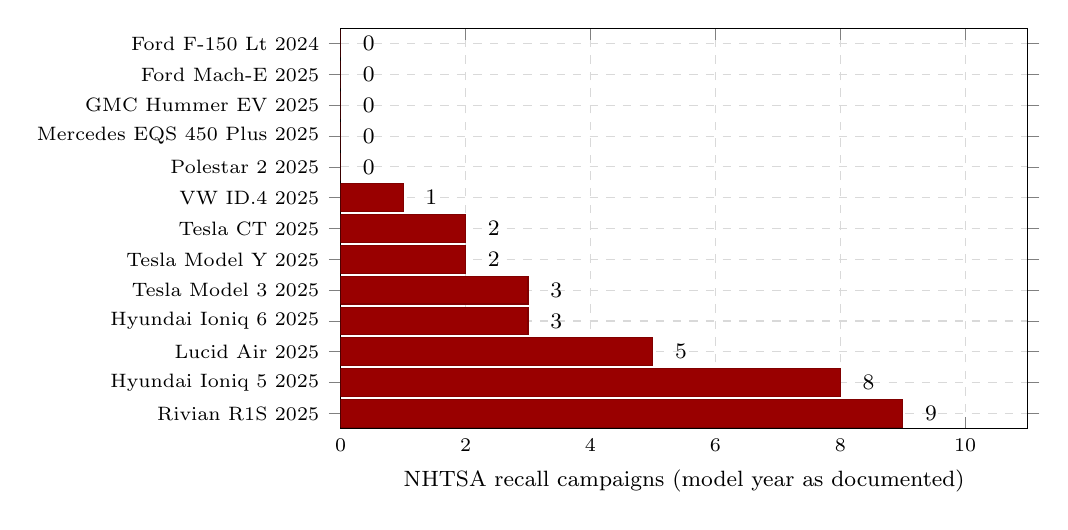
\begin{tikzpicture}
  \begin{axis}[
      width=0.85\textwidth, height=0.55\textwidth,
      xbar, xmin=0, xmax=11,
      ymin=0.5, ymax=13.5,
      ytick={1,2,3,4,5,6,7,8,9,10,11,12,13}, yticklabels={Rivian R1S 2025,Hyundai Ioniq 5 2025,Lucid Air 2025,Hyundai Ioniq 6 2025,Tesla Model 3 2025,Tesla Model Y 2025,Tesla CT 2025,VW ID.4 2025,Polestar 2 2025,Mercedes EQS 450 Plus 2025,GMC Hummer EV 2025,Ford Mach-E 2025,Ford F-150 Lt 2024},
      xlabel={NHTSA recall campaigns (model year as documented)},
      tick label style={font=\scriptsize},
      xlabel style={font=\footnotesize},
      bar width=10pt,
      nodes near coords align={horizontal},
      grid=major, grid style={dashed,gray!30},
    ]
    \addplot[fill=red!60!black, draw=red!50!black] coordinates {(9,1) (8,2) (5,3) (3,4) (3,5) (2,6) (2,7) (1,8) (0,9) (0,10) (0,11) (0,12) (0,13)};
    \node[anchor=west, font=\footnotesize] at (axis cs:9.2,1) {9};
    \node[anchor=west, font=\footnotesize] at (axis cs:8.2,2) {8};
    \node[anchor=west, font=\footnotesize] at (axis cs:5.2,3) {5};
    \node[anchor=west, font=\footnotesize] at (axis cs:3.2,4) {3};
    \node[anchor=west, font=\footnotesize] at (axis cs:3.2,5) {3};
    \node[anchor=west, font=\footnotesize] at (axis cs:2.2,6) {2};
    \node[anchor=west, font=\footnotesize] at (axis cs:2.2,7) {2};
    \node[anchor=west, font=\footnotesize] at (axis cs:1.2,8) {1};
    \node[anchor=west, font=\footnotesize] at (axis cs:0.2,9) {0};
    \node[anchor=west, font=\footnotesize] at (axis cs:0.2,10) {0};
    \node[anchor=west, font=\footnotesize] at (axis cs:0.2,11) {0};
    \node[anchor=west, font=\footnotesize] at (axis cs:0.2,12) {0};
    \node[anchor=west, font=\footnotesize] at (axis cs:0.2,13) {0};
  \end{axis}
\end{tikzpicture}

\caption{NHTSA recalls for the documented model year, by product. Rivian R1S, Hyundai Ioniq 5, and Lucid Air dominate; quality-marketing language does not, in general, reflect first-year defect-discovery rate.}
\label{fig:recall-bars}
\end{figure}
\FloatBarrier

% =================================================================== %
\section{Limitations and Threats to Validity}\label{sec:limits}

This dataset is v0.1 and the sample is small ($n=13$ products). We explicitly do not claim the findings generalize to the full US EV market; that requires a randomized expansion (Phase 2). Specific limitations:

\begin{enumerate}
  \item \textbf{Selection bias}: Products were chosen partly because Consumer Reports had documented large gaps for them. Phase 2 will randomize within the top-15 US-sales list.
  \item \textbf{Single-unit Tier-2 testing}: CR, Edmunds, MotorTrend tests typically use $N=1$ purchased unit. We mitigate by triangulating across publishers when possible.
  \item \textbf{Software-update drift}: EVs receive OTA updates that materially affect range/charging behavior. Records timestamp \texttt{last\_verified}; re-verification is required at $\geq 12$ month intervals.
  \item \textbf{Manufacturer perspective absent}: No manufacturer was contacted for response. The dataset is, in v0.1 form, one-sided. A pre-publication notification template for $\geq 30$-day manufacturer response is included in the repository.
  \item \textbf{Source-reproducibility risk}: Some Tier-2 sources (CR) are partly paywalled; some Tier-4 manufacturer URLs change without warning. We mitigate via verbatim quotes and web.archive.org snapshots, but link rot is real.
  \item \textbf{Inter-rater reliability not yet measured}: Tactic assignments were performed by a single annotator. Cohen's $\kappa$ on a sample of 20 records is a Phase~2 deliverable.
\end{enumerate}

% =================================================================== %
\section{Conclusion and Future Work}\label{sec:conclusion}

DataDeception is a methodology-and-dataset for systematically documenting commercial-claims deception, instantiated for the U.S.\ electric-vehicle market. The contribution is primarily the \emph{method}: a citation-first schema with mandatory tier-classified sources, an open tactic taxonomy with cross-manufacturer corroboration thresholds, and an evidence-grade rubric that admits replication. The v0.1 dataset is small but supports preliminary RQ1 and RQ2 testing and demonstrates the feasibility of a public, schema-validated artifact in this space.

Phase 2 work prioritizes: randomized expansion to 25+ products, longitudinal re-verification, manufacturer-response integration, inter-rater reliability measurement, and instantaneous-snapshot pipeline for Tier-4 manufacturer URLs. The dataset and methodology generalize beyond EVs; we anticipate parallel instantiations for televisions (subject to RTINGS access constraints), laptops (Notebookcheck), and audio (Audio Science Review). The same schema applies; only the source-tier-2 base differs.

\paragraph{Reproducibility statement.} All artifacts are available at \url{https://github.com/Princeu3/DataDeception} under MIT (code) and CC-BY-4.0 (data). The figure-generation pipeline is deterministic and reads only the JSON dataset; running \texttt{paper/figures/generate.py} reproduces all auto-derived figures. Schema validation is via \texttt{validate.py} (one command, exits non-zero on any integrity violation).

\paragraph{Acknowledgements.} This work was supported by Claude (Anthropic) as a research-pair-programming partner during data curation, schema iteration, and figure-pipeline development. All judgment calls about evidence grading, tactic naming, and limitation framing were made by the human author and are auditable in the public Git history.

\bibliographystyle{plainnat}
\bibliography{references}

\end{document}
